\documentclass[main.tex]{subfiles}
\begin{document}

\chapter{Background}
%------------------
\section{Modeling Mechanical Systems}
\subsection{Lagrangian Mechanics}
Robotic systems may have complex movement ranges, combining various types of rotations, translations, or extensions. Attempting to model each joint of a robot as a coordinate of three-space (some subset of $\ree^3$) can quickly become a mess of trigonometry. This motivates control systems engineers to instead model the robot's \textbf{configuration space} as a manifold $Q$, so that any configuration of the robot is an element of the Cartesian product of its joints' own configuration spaces.

Each coordinate $q^i$ of a point $q\in Q$ is called a \textbf{generalized coordinate}. The number of coordinates corresponds to the robot's degrees of freedom.

A system can be modelled with the generalized coordinates $q\in Q$ using Lagrangian mechanics. This motivates the following definition.
\begin{boxdef}{Smooth Simple Mechanical System \cite{bullo2019geometric}}
A set $\del{Q,\mathbb{G},P}$, where
\begin{enumerate}[i.]
    \item $Q$ is a smooth manifold called the configuration manifold. This is the manifold whose points consist of all possible coordinate configurations of the system.
    \item $\mathbb{G}$ is a smooth Riemannian metric on $Q$ called the kinetic energy metric, typically defined as $\mathbb{G}(q,\dot q)=\frac{1}{2}\dot q^T D(q) \dot q$.
    \item $P$ is a smooth potential function on $Q$. This may be a gravitational potential, but other potentials are common as well.
\end{enumerate}
\end{boxdef}\label{def:system}
This definition will be expanded to a Smooth Simple Mechanical Control System in \ref{def:controlsystem}.

\subsection{Holonomic Constraints}
A system may be subject to constraints:
a set of restrictions imposed on its possible velocity and positional configurations. 
\textbf{Holonomic contraints} are one class of constraint acting purely on the spatial (and time) coordinates of a system, but not on the velocity coordinates. Additionally, holonomic constraints can be written as a homogeneous equation.

A simple example is a point particle that is restricted to the surface of a sphere with radius $R$. Subject to this constraint, the point's spatial coordinates $(x,y,z)$ are required to satisfy the equality
\begin{align}
    x^2+y^2+z^2=R^2.
\end{align}
This is an example of a holonomic constraint, because we are able to define the constraint as a uniformly homogeneous function of the spatial coordinates (and time). Define the constraint $h$ as:
\begin{align}
    h(x,y,z,t):=x^2+y^2+z^2-R^2\equiv 0.
\end{align}
Note that the constraint is independent of velocity, and is therefore \textit{holonomic} by definition.

On the other hand, constraining that particle to the {interior} of the sphere would be an example of a \textbf{non-holomic constraint}. 
\begin{align}
    x^2+y^2+z^2<R^2 \implies h(x,y,z,t):=x^2+y^2+z^2-R^2<0\qq{and therefore}h\neq 0.
\end{align}
While the constraint depends only on spatial coordinates, it cannot be expressed as an identically homogeneous function, which disqualifies it from being holonomic.

\subsection{Virtual Holonomic Contraints }\label{vhc-section}
In this study, we are especially interested in artificially imposing holonomic constraints on mechanical systems by means of control. \textbf{Virtual holonomic constraints}, as they are called, are not ``true" constraints on the system--the controller acts on the system's actuators to make the system \textit{appear} to be holonomically constrained. Of course, disabling the controller would allow the system to move in its natural, unconstrained fashion.

As a practical example, a Virtually Holonomic Constrained system could look like matching joint angles on a group of several identical robots such that they all walk in formation\cite{maggiore2012virtual}. Suppose $\theta_i$ describes the $i$\textsuperscript{th} robot's knee joint angle. If all robots walk in formation, all of their knee joints should be commanded to match some angle $\Theta(t)$. The VHC would therefore be written as,
\begin{align}
    h(\theta):=\sum_i \theta^i-\Theta(t)\equiv 0.
\end{align}
As a second example, modern vehicles are often equipped with advanced cruise control systems, which allow a driver to configure their vehicle to follow a set distance behind the vehicle ahead of them. This makes the two vehicles appear to be holonomically constrained (the norm of the difference between the vehicles' position vectors is constant), and this constraint is artifically enforced by the cruise controller.

Maggiore and Consolini provide a formal definition for VHCs, as well as an overview of the conditions under which they can be imposed\cite{maggiore2012virtual}.

\begin{boxdef}{Virtual Holonomic Constraint \cite{maggiore2012virtual}}
For a smooth simple mechanical control system $\del{Q,\mbbg,P,F}$ as defined in Definition \ref{def:controlsystem}, a virtual holonomic constraint of order $k$ is a smooth relation $h:Q\to\ree^k$,
$h(q)={0}$, and for all $q\in h\inv(0),$ and the constraint manifold
\begin{align}
    \mathcal{C}=\cbr{(q,\qd):h(q)=0,\dd h_q\cdot\qd=0}
\end{align}
is controlled invariant. That means, there exists a smooth feedback $\tau(q,\qd)$ that enforces the constraint, such that $\mathcal{C}$ is (asymptotically) invariant.
\end{boxdef}
It is important to ensure a chosen VHC is well-defined and well-behaved.
\begin{boxthm}{Conditions for regular VHCs \cite{maggiore2012virtual}}
Let $h:Q\to\ree^n$ be smooth, $\rank \dd h_q=k$ for all $q\in h\inv(0).$ Then $h(q)$ is a \textbf{regular VHC of order $k$} if and only if $\forall q\in h\inv(0),$
\begin{align}
     \dim\sbr{Im(D\inv(q)B(q))\cap \Ker{\dhq}}=n-1-k.
\end{align}
\end{boxthm}\label{thm:regularvhc}
For the purpose of the dynamical reduction technique, we want select a set of VHCs that respect the symmetry of the given mechanical system. 

\subsection{Symmetry}
This project considers mechanical systems endowed with one symmetry. A precise definition follows.
\begin{boxdef}{Symmetry 
\cite{bullo2019geometric}%591
}
Let $\del{Q,\mbbg,P}$ be a smooth simple mechanical system. \begin{enumerate}[(a)]
    \item\label{def:lagr-invariant} A smooth left action $\Phi$ of a Lie group $G$ on $Q$ is a \textbf{symmetry} of the system if $\Phi$ is an isometry of $(Q,\mathbb{G})$ and $F,P$ are $\Phi$-invariant. In other words, the kinetic metric $\mathbb{G}$ and the potential and control forces are invariant under the action of $\Phi$.
    \item A smooth vector field $X$ on $Q$ is an \textbf{infinitesimal symmetry} of the system is $X$ is an infinitesimal isometry, and $P$ is $X$-invariant.
\end{enumerate}
\end{boxdef}\label{def:symmetry}
A noteworthy extension of \ref{def:lagr-invariant} above is that the Lagrangian $\Lagr(\qd,q)$ is also invariant under the action of $\Phi$. This leads to Noether's Theorem, one of the key findings of 20\textsuperscript{th} century physics.

\begin{boxthm}{Noether's Theorem (simplified) \cite{bullo2019geometric}%292
}
Let $\del{Q,\mbbg,P}$ be a smooth simple mechanical system, and let $\gamma:I\to Q$ be a solution to its equations of motion, and $J$ is the conserved quantity (momentum map) with respect to the symmetry. Then
\begin{enumerate}[(a)]
    \item if $\Phi:G\cross Q\to Q$ is a symmetry, then for all $\zeta\in g$,
    \begin{align}
        \dv{}{t}\langle J_\Phi(t,\gamma'(t)),\zeta\rangle
        =
        0.
    \end{align}
    \item  if $X$ is an infinitesimal symmetry, then
    \begin{align}
        \dv{}{t} J_X(\gamma'(t))
        =
        0.
    \end{align}
\end{enumerate}
\end{boxthm}

% \subsection{Constrained Dynamics}
% \todo[inline]{Work in progress}
% Given the system dynamics and a set of regular VHCs, the constrained dynamics can be derived. The system is parametrized in terms of the VHCs, so that its dynamics lie entirely within the constraint set $\mathcal{C}$:
% \begin{align}
%     \ddot{\vec{s}}=\vec{f}(\dot{\vec{s}}, \vec{s})
% \end{align}

\section{Control Systems}
\subsection{Anatomy of a Control System}
A \textbf{feedback control system} is a system that can be dynamically steered towards some desired target state, based on iterative feedback of its current state\cite{franklin2002feedback}.

In control theory terminology, a \textbf{plant} is the part of the system that is being controlled--likely a robot in this context. The purpose of the control system is to push the robot towards a goal element or submanifold of the configuration manifold, known as a \textbf{reference signal} $r(t)$.

A \textbf{sensor} measures the variable of interest $y(t)$ on the plant. The sensor allows the system to perceive its current state, and then pass these measurements to the controller\cite{franklin2002feedback}. 

The \textbf{controller} itself is the brain of the system: its goal is to process the sensor inputs, and then output a command signal corresponding to the discrepancy between the reference state and the current state. This difference, $e(t):=r(t)-y(t)$, is called the \textbf{error}. The controller's outputted command signal $u(t)$ informs behaviour of the actuator(s) in the plant, resulting in the system's iterative convergence towards the desired state $r(t).$

A controller is generally designed and tuned to meet a set of requirements\cite{franklin2002feedback}, which can include minimizing $e(t)$ as quickly as possible, minimizing oscillations during convergence towards $r(t)$, maintaining stability under disturbances, maintaining stability on a large subset of $Q$, or minimizing the robot's energy cost of the control forces while still approaching $r(t)$.

Figure \ref{fig:feedback} shows the flow of information through a feedback control system.
\begin{figure}[h]
    \centering
    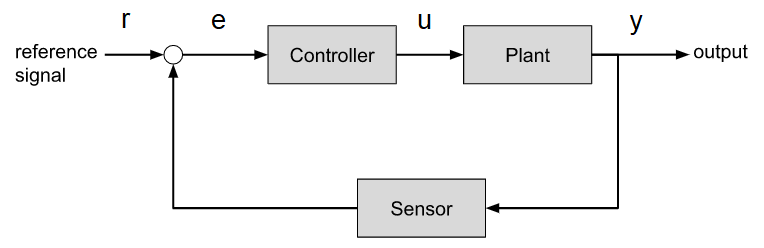
\includegraphics[width=0.75\columnwidth]{assets/feedback-modified.png}
    \caption{Block diagram of a simple feedback control system}
    \label{fig:feedback}
\end{figure}



\subsection{Smooth Simple Mechanical Control Systems}
Definition \ref{def:system} must now be revised with the addition of another object: the control force. 
The configuration manifold $Q$ is the set of possible states that the plant can occupy.
Each actuator in the plant outputs a torque or force given by $\tau_i$, mathematically modeled as a covector field on $Q$. 
\begin{boxdef}{Smooth Simple Mechanical Control System \cite{bullo2019geometric}}
A set $\del{Q,\mathbb{G},P,F}$, where
\begin{enumerate}[(a)]
    \item $Q$ is a smooth manifold called the configuration manifold. This is the manifold whose points consist of all possible coordinate configurations of the system.
    \item $\mathbb{G}$ is a smooth Riemannian metric on $Q$ called the kinetic energy metric, typically defined as $\mathbb{G}(q,\dot q)=\frac{1}{2}\dot q^T D(q) \dot q$, where $D(q)$ is the intertia matrix.
    \item $P$ is a smooth potential function on $Q$. This may be a gravitational potential, but other potentials are common as well.
    \item $F=\cbr{\tau_1,\tau_2,\ldots,\tau_k}$ is a set of covector fields on $Q$ representing the control forces generated by each actuator on the system.
\end{enumerate}
\end{boxdef}\label{def:controlsystem}
This is the only type of control systems considered through this project.

% The tangent bundle of $\mathcal{C}$

\subsection{Modelling a Smooth Simple Mechanical Control System}
Putting all the pieces together, a generalized differential equation for a simple mechanical control system is given by:
\begin{align}
    D\del{ q}\qdd+C\del{ q,\qd}\qd+\nabla_qP\del{ q}=B\tau\label{control-equation}
\end{align}
where each variable is defined as follows:%\todo{I want to add what type of mathematical object each variable is}
\begin{enumerate}[(a)]
    \item $q$ is the generalized coordinate vector at the point $q\in Q$ of the system, and $\qd,\qdd$ are the respective first and second time derivatives of $q$.
    \item $D(q)$ (also known as $M(q)$) is the inertia matrix describing the system's mass and intertia in each coordinate direction.
    \item $C\del{q,\qd}$ is the Coriolis matrix.
    \item $P\del{q}$ is a scalar function whose gradient with respect to the generalized coordinate vector $q$ describes the potential field of the system.
    \item $B$ is a $\del{\dim q }\cross\del{ \dim \tau}$ matrix, which relates the degrees of freedom of the system to the number of control inputs. For example, if the system is characterized by 4 generalized coordinates and 2 actuators, $B\in M_{4\cross 2}\del{\ree}$.
    \item $\tau$ is the vector containing the elements of $F$ (set of control inputs of the system described in Definition \ref{def:controlsystem}).
\end{enumerate}
Constraints are expressed as a vector function, ${h}(q)$,
    \begin{align}
        {h}(q)&=\pmqty{h_1(q)\\h_2(q)\\\vdots}\equiv \vec{0}.
    \end{align}
    \subsection{Control Error}
    Since the goal is to drive the holonomic constraints to zero through control, it makes sense to equate the VHC with the error:
    \begin{align} e( q):= h( q).
    \end{align}
   From here, the corresponding time derivatives of the Error are found (omitting vector symbols for simplicity):
    \begin{align}
    &\begin{aligned}
        {e}&= h( q);
    \end{aligned}\\
    &\begin{aligned}
    \dot{{e}}&=\dv{}{t} h( q)\\&=\dd {h}({q})\dot{{q}};\\
    \end{aligned}\\
    &\begin{aligned}
    \ddot{{e}}&=\dv{}{t}\del{\dd {{h}({q})}\dot{{q}}}\\
    &=\dot{{q}}^\top\del{\pdv{}{ q}\grad_q{{h}({q})}}\dot{{q}}+\dd {{h}({q})}\ddot{{q}}.\label{eq:edd}
    \end{aligned}
    \end{align}
    Where $\dhq$ is the Jacobian operator on $h$, as defined in \ref{def:jacobian}.
    
    \subsection{Control Law}
    By isolating for $\ddot{ q}$ in Equation \ref{eq:edd}, we can set $\ddot{{e}}$ as a function of our control, $\tau$. Then, we can choose the control, $\tau$, so that it drives $\ddot{{e}}\to \vec{0}$. Starting from Equation \ref{control-equation},
    \begin{align}
        \ddot{{q}}=D\inv({q})\del{B{\tau}
        -C\del[1]{ q,\qd}\qd-\nabla_qP\del{ q}}.\label{eq:qdd}
    \end{align}
    Substitute Equation \ref{eq:qdd} into Equation \ref{eq:edd}), and assuming that $\ddot{{e}}$ is driven to zero, we can isolate for ${\tau}$ to obtain the \textbf{Control law}:
    \begin{align}
    \begin{aligned}
        {\tau}&=\beta\del{-\pdv{h(q)}{t}+\dhq
        D\inv\del{C(q,\qd)\qd+G(q)}-K_Pe-K_D\dot{e}};\\
        &\qq{where}\beta:=\del{\dhq D\inv B}\inv.
        %tau = beta*(-dhqdt_num+dhq_num*inv(D_num)*(C_num+G_num) -Kp*e-Kd*edot); 
        %beta = inv(dhq_num*(D_num\B));
    \end{aligned}\label{eq:controllaw}
    \end{align}
Here, a PD-style controller is used. These are easy to tune and implement, and have stood the test of time across industries\cite{franklin2002feedback}.
The parameters $K_P,K_D$ are the proportional and derivative controller parameters. These are chosen by the control system designer to meet whichever requirements are defined for satisfactory performance.


\section{Concepts of Differential Geometry}
% \todo[inline]{Work in progress.}
% \begin{boxdef}{Covariant Derivative}
    
% \end{boxdef}
% \begin{boxdef}{Parallel Transport}
    
% \end{boxdef}
While the natural basis elements of $\ree^n$ are invariant throughout $\ree^n$, this is not generally the case on manifolds.
\begin{boxdef}{Christoffel Symbol}\label{eq:christoffel}
Christoffel symbols are real numbers that describe how the basis element of a manifold transforms at each point on the manifold. 

The $(i,j,k)$\textsuperscript{th} Christoffel Symbol of the second kind is a real number $\Gamma^k_{ij}:Q\to\ree$ defined by:
\begin{align}
   \Gamma^k_{ij}:=\frac{1}{2}\sum_{l=1}^n D\inv_{kl}\del{\pdv{D_{jl}}{q_i}+\pdv{D_{il}}{q_j}-\pdv{D_{ij}}{q_l}},\\\qq{for} i,j,k\in\cbr{1,2,\ldots,n}. 
\end{align}
Here, $D_{ij},D\inv_{ij}$ denote the $(i,j)$\textsuperscript{th} matrix elements of the inertia matrix $D(q)$ and its inverse, respectively.
\end{boxdef}

The constrained dynamics have their own respective Christoffel symbols, which account for the parametrization $q=\varphi(s)$.
\begin{boxdef}{Christoffel Symbols of the Constrained Connection}\label{eq:christoffelconstrained}
The $(i,j,k)$\textsuperscript{th} Christoffel Symbol corresponding to the constrained connection $\nablac$ is a real number $\Gammac{k}{ij}:Q\to\ree$ defined by:
\begin{align}
   \Gammac{k}{ij}:=\sum^n_{a=1}
   \sbr{(B^\bot D\dd\varphi_s)\inv B^\bot D}_{ka}
   \del{\pdv{\varphi^a}{s^i}{s^j}+\del{\pdv{\varphi}{s^i}^\top}\Gamma^a\del{\pdv{\varphi}{s^j}}}\eval{q=\varphi(s)}
   ,\\\qq{for} i,j,k\in\cbr{1,2,\ldots,n-m}. 
\end{align}
Here, $D_{ij},D\inv_{ij}$ denote the $(i,j)$\textsuperscript{th} matrix elements of the inertia matrix $D(q)$ and its inverse, respectively.
\end{boxdef}
% \begin{boxdef}{Ehresmann connection}\label{def:ehresmann}
    
% \end{boxdef}


\end{document}